\documentclass{beamer}
\usepackage{amsmath}
\usepackage[english]{babel} %set language; note: after changing this, you need to delete all auxiliary files to recompile
\usepackage[utf8]{inputenc} %define file encoding; latin1 is the other often used option
\usepackage{csquotes} % provides context sensitive quotation facilities
\usepackage{graphicx} %allows for inserting figures
\usepackage{booktabs} % for table formatting without vertical lines
\usepackage{textcomp} % allow for example using the Euro sign with \texteuro
\usepackage{stackengine}
\usepackage{wasysym}
\usepackage{tikzsymbols}
\usepackage{textcomp}
% ELIMINAR COMANDOS DE NAVEGACION%%%%%%%%%%%
\setbeamertemplate{navigation symbols}

%\newcommand{\bubblethis}[2]{
 %       \tikz[remember picture,baseline]{\node[anchor=base,inner sep=0,outer sep=0]%
 %       (#1) {\underline{#1}};\node[overlay,cloud callout,callout relative pointer={(0.2cm,-0.7cm)},%
 %       aspect=2.5,fill=yellow!90] at ($(#1.north)+(-0.5cm,1.6cm)$) {#2};}%
 %   }%
%\tikzset{face/.style={shape=circle,minimum size=4ex,shading=radial,outer sep=0pt,
 %       inner color=white!50!yellow,outer color= yellow!70!orange}}

%% Some commands to make the code easier
\newcommand{\emoticon}[1][]{%
  \node[face,#1] (emoticon) {};
  %% The eyes are fixed.
  \draw[fill=white] (-1ex,0ex) ..controls (-0.5ex,0.2ex)and(0.5ex,0.2ex)..
        (1ex,0.0ex) ..controls ( 1.5ex,1.5ex)and( 0.2ex,1.7ex)..
        (0ex,0.4ex) ..controls (-0.2ex,1.7ex)and(-1.5ex,1.5ex)..
        (-1ex,0ex)--cycle;}
\newcommand{\pupils}{
  %% standard pupils
  \fill[shift={(0.5ex,0.5ex)},rotate=80] 
       (0,0) ellipse (0.3ex and 0.15ex);
  \fill[shift={(-0.5ex,0.5ex)},rotate=100] 
       (0,0) ellipse (0.3ex and 0.15ex);}

\newcommand{\emoticonname}[1]{
  \node[below=1ex of emoticon,font=\footnotesize,
        minimum width=4cm]{#1};}
\usepackage{scalerel}
\usetikzlibrary{positioning}
\usepackage{xcolor,amssymb}
\newcommand\dangersignb[1][2ex]{%
  \scaleto{\stackengine{0.3pt}{\scalebox{1.1}[.9]{%
  \color{red}$\blacktriangle$}}{\tiny\bfseries !}{O}{c}{F}{F}{L}}{#1}%
}
\newcommand\dangersignw[1][2ex]{%
  \scaleto{\stackengine{0.3pt}{\scalebox{1.1}[.9]{%
  \color{red}$\blacktriangle$}}{\color{white}\tiny\bfseries !}{O}{c}{F}{F}{L}}{#1}%
}
\usepackage{fontawesome} % Social Icons
\usepackage{epstopdf} % allow embedding eps-figures
\usepackage{tikz} % allows drawing figures
\usepackage{amsmath,amssymb,amsthm} %advanced math facilities
\usepackage{lmodern} %uses font that support italic and bold at the same time
\usepackage{hyperref}
\usepackage{tikz}
\hypersetup{
    colorlinks=true,
    linkcolor=blue,
    filecolor=magenta,      
    urlcolor=blue,
}
\usepackage{tcolorbox}
%add citation management using BibLaTeX
\usepackage[citestyle=authoryear-comp, %define style for citations
    bibstyle=authoryear-comp, %define style for bibliography
    maxbibnames=10, %maximum number of authors displayed in bibliography
    minbibnames=1, %minimum number of authors displayed in bibliography
    maxcitenames=3, %maximum number of authors displayed in citations before using et al.
    minnames=1, %maximum number of authors displayed in citations before using et al.
    datezeros=false, % do not print dates with leading zeros
    date=long, %use long formats for dates
    isbn=false,% show no ISBNs in bibliography (applies only if not a mandatory field)
    url=false,% show no urls in bibliography (applies only if not a mandatory field)
    doi=false, % show no dois in bibliography (applies only if not a mandatory field)
    eprint=false, %show no eprint-field in bibliography (applies only if not a mandatory field)
    backend=biber %use biber as the backend; backend=bibtex is less powerful, but easier to install
    ]{biblatex}
\addbibresource{../mybibfile.bib} %define bib-file located one folder higher


\usefonttheme[onlymath]{serif} %set math font to serif ones

\definecolor{beamerblue}{rgb}{0.2,0.2,0.7} %define beamerblue color for later use

%%% defines highlight command to set text blue
\newcommand{\highlight}[1]{{\color{blue}{#1}}}


%%%%%%% commands defining backup slides so that frame numbering is correct

\newcommand{\backupbegin}{
   \newcounter{framenumberappendix}
   \setcounter{framenumberappendix}{\value{framenumber}}
}
\newcommand{\backupend}{
   \addtocounter{framenumberappendix}{-\value{framenumber}}
   \addtocounter{framenumber}{\value{framenumberappendix}}
}

%%%% end of defining backup slides

%Specify figure caption, see also http://tex.stackexchange.com/questions/155738/caption-package-not-working-with-beamer
\setbeamertemplate{caption}{\insertcaption} %redefines caption to remove label "Figure".
%\setbeamerfont{caption}{size=\scriptsize,shape=\itshape,series=\bfseries} %sets figure  caption bold and italic and makes it smaller


\usetheme{Boadilla}

%set options of hyperref package
\hypersetup{
    bookmarksnumbered=true, %put section numbers in bookmarks
    naturalnames=true, %use LATEX-computed names for links
    citebordercolor={1 1 1}, %color of border around cites, here: white, i.e. invisible
    linkbordercolor={1 1 1}, %color of border around links, here: white, i.e. invisible
    colorlinks=true, %color links
    anchorcolor=black, %set color of anchors
    linkcolor=beamerblue, %set link color to beamer blue
    citecolor=blue, %set cite color to beamer blue
    pdfpagemode=UseThumbs, %set default mode of PDF display
    breaklinks=true, %break long links
    pdfstartpage=1 %start at first page
    }


% --------------------
% Overall information
% --------------------
\title[Economía I]{Economía I \vspace{4mm}
\\ Magistral 11: Competencia perfecta}
\date{}
\author[Ertola Navajas y Fariña]{Ertola Navajas y Fariña}
\vspace{0.4cm}
\institute[]{Universidad de San Andrés} 

\begin{document}

\begin{frame}
\titlepage
\centering

\includegraphics[scale=0.2]{Slides Principios de Economia/Figures/logoUDESA.jpg} 
\end{frame}


\begin{frame}
\frametitle{¿Se acuerdan del equilibrio de mercado?}
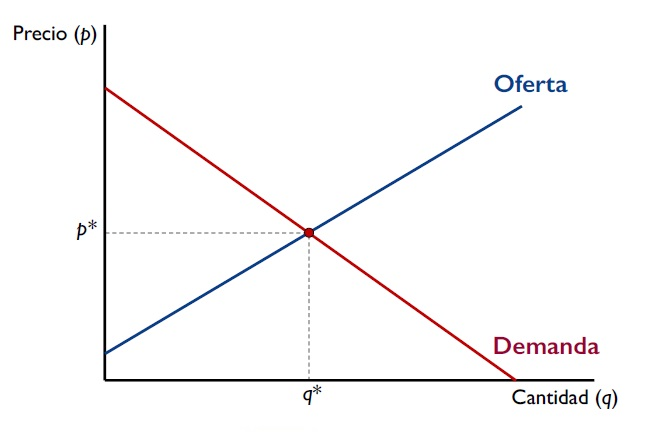
\includegraphics[scale=0.6]{Slides Principios de Economia/Figures/Tema_07.3_equilibrioofertademanda_0.jpg}
\end{frame}

\begin{frame}
\frametitle{Equilibrio}
\begin{itemize}
    \item En el precio de equilibrio (market-clearing price), la oferta iguala a la demanda.\vspace{4mm}
    \item Otros precios no son un equilibrio de Nash\vspace{2mm}
    \begin{itemize}
        \item Si p $>$ p*, entonces habría exceso de oferta \\\vspace{1mm}
        \item Si p $<$ p*, entonces habría exceso de demanda \\\vspace{1mm}
        \item Se asume que los productos son idénticos, por lo que los compradores estarían dispuestos a comprar a cualquier vendedor
    \end{itemize}
\end{itemize}
\end{frame}

\begin{frame}
\frametitle{Tipos de mercado}
\begin{itemize}
    \item ¿Que tipo de mercado vamos a estudiar?\vspace{2mm}
    \begin{enumerate}
        \item Competencia perfecta\vspace{1mm}
        \item Competencia Monopolistica\vspace{1mm}
        \item Oligopolio\vspace{1mm}
        \item Monopolio \vspace{1mm}
    \end{enumerate}
\end{itemize}
\end{frame}

\begin{frame}
\frametitle{Competencia y empresas tomadoras de precios}
\begin{itemize}
    \item ¿Cuándo tenemos una mercado competitivo?\vspace{2mm}
    \begin{enumerate}
        \item Muchos compradores y vendedores no diferenciados que actúan en forma independiente.\vspace{1mm}
        \item El precio viene determinado por el mercado.\vspace{1mm}
        \item Productos ofrecidos básicamente idénticos.\vspace{1mm}
        \item Información perfecta de los consumidores y las empresas.\vspace{1mm}
        \item Las firmas entran o salen del mercado libremente.
    \end{enumerate}
    \vspace{2mm}
    \item En un mercado competitivo las firmas y los consumidores son tomadores de precios.\vspace{2mm}
    \begin{itemize}
        \item Para la firma esto quiere decir que el precio de mercado es igual al ingreso marginal \\
        - ¿Por qué?
    \end{itemize}
\end{itemize}
\end{frame}

\begin{frame}
\frametitle{Precios determinados por el mercado}
\begin{itemize}
    \item Las firmas son tomadoras de precios, eso quiere decir que no pueden:\vspace{2mm}
    \begin{itemize}
        \item Influir en el precio de mercado.\vspace{1mm}
        \item Beneficiarse de la elección de un precio diferente del precio de mercado.\vspace{2mm}
    \end{itemize}
    \item Ingreso Marginal = Precio = Ingreso Medio ($ \frac{(PxQ)}{Q}$)\vspace{2mm}
    \item La curva de demanda (conjunto factible) de estas firmas se vuelve completamente plana.\vspace{2mm}
    \item La curva de oferta es la curva de CMg de la firma.
    \end{itemize}
    \begin{center}
        \textbf{La empresa elige cantidad, no precio}
    \end{center}
\end{frame}

%\begin{frame}
%\frametitle{Demanda de mercado vs Demanda de la empresa}
%\end{frame}

\begin{frame}
\frametitle{¿Qué pasa en la empresa?}
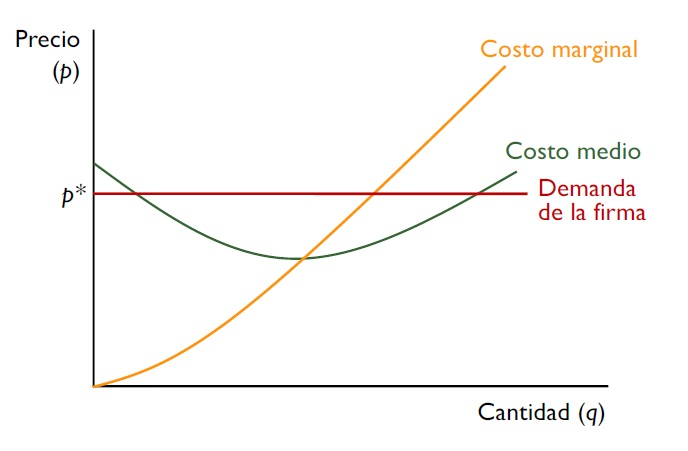
\includegraphics[scale=0.6]{Slides Principios de Economia/Figures/Tema_07.7_compperfecta.jpg}
\end{frame}

\begin{frame}
\frametitle{¿Qué pasa si el precio es mayor que el costo marginal?}
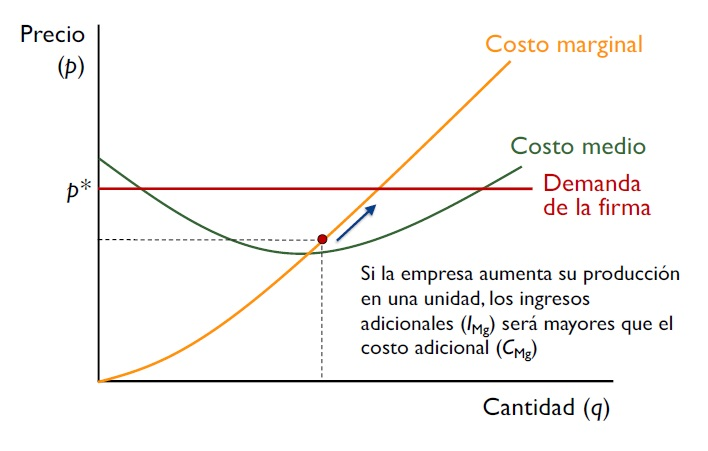
\includegraphics[scale=0.55]{Slides Principios de Economia/Figures/Tema_07.8_compperfecta2.jpg}
\end{frame}

\begin{frame}
\frametitle{¿Qué pasa si el precio es menor que el costo marginal?}
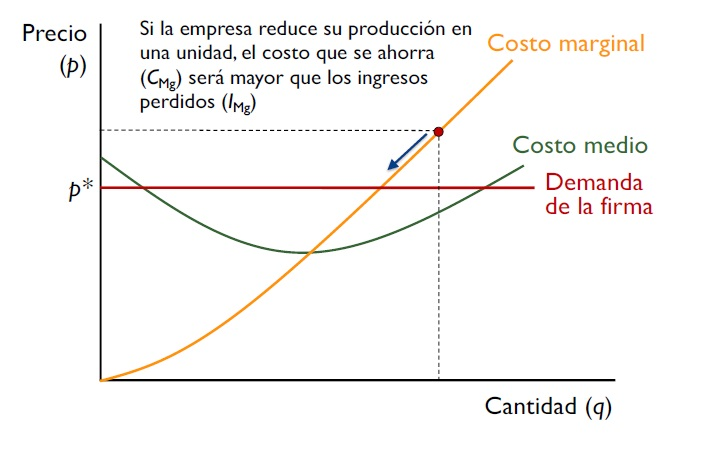
\includegraphics[scale=0.55]{Slides Principios de Economia/Figures/Tema_07.9_compperfecta3.jpg}
\end{frame}

\begin{frame}
\frametitle{La empresa maximiza beneficios, ¿cómo?}
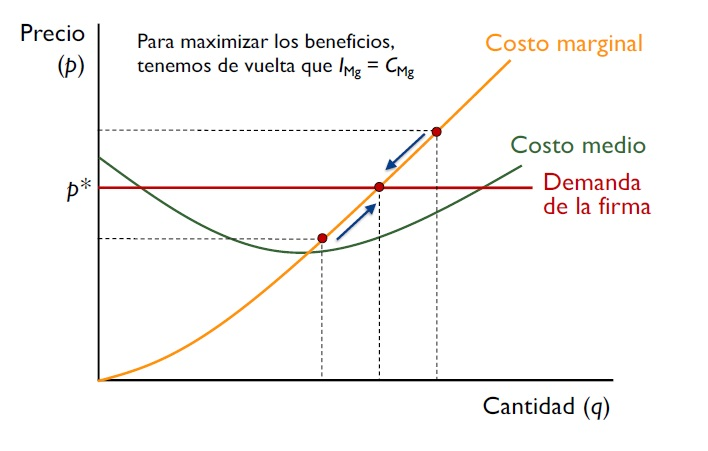
\includegraphics[scale=0.55]{Slides Principios de Economia/Figures/Tema_07.10_compperfecta4.jpg}
\end{frame}

\begin{frame}
\frametitle{Veamos un ejemplo}
\begin{itemize}
    \item Precio: \$32
    \item Costo marginal = $2Q^{2}$
\end{itemize}
\centering
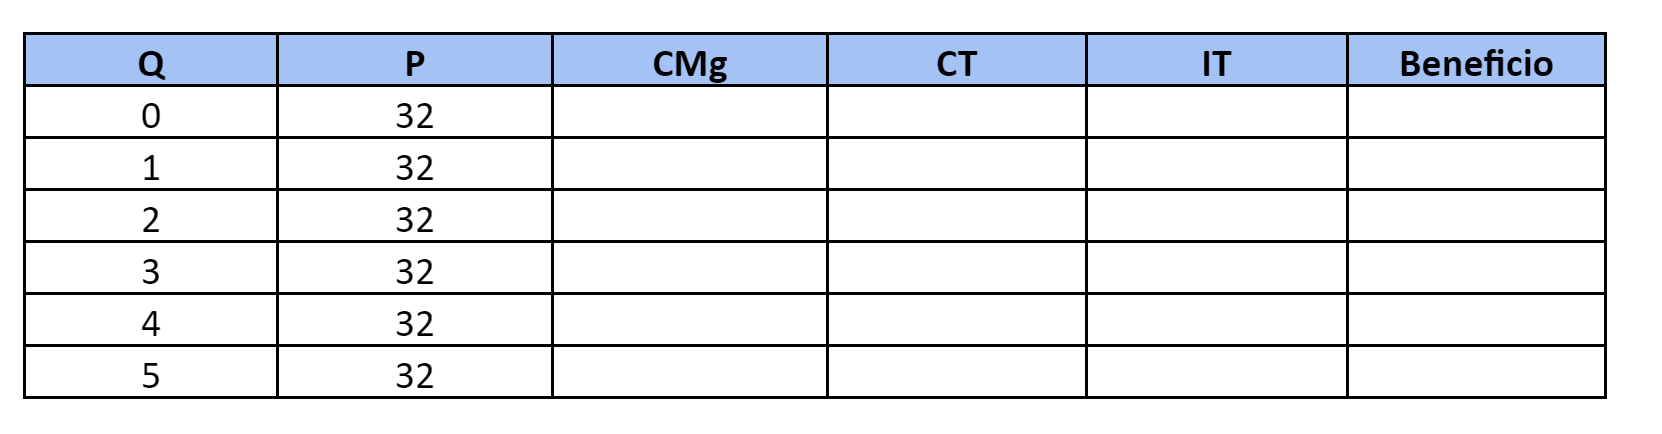
\includegraphics[scale=0.7]{Slides Principios de Economia/Figures/Ejemplo Competencia Perfecta.png}
\end{frame}

\begin{frame}
\frametitle{Si lo graficamos....}
\centering
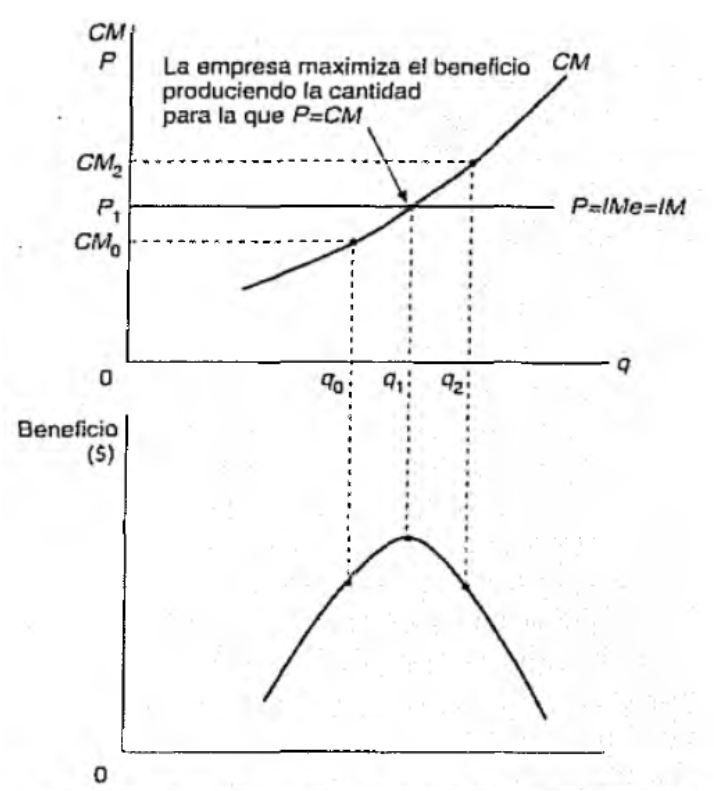
\includegraphics[scale=0.85]{Slides Principios de Economia/Figures/BeneficiosCP.png}
\end{frame}

\begin{frame}
\frametitle{¿Habrá beneficio en este punto? SI!}
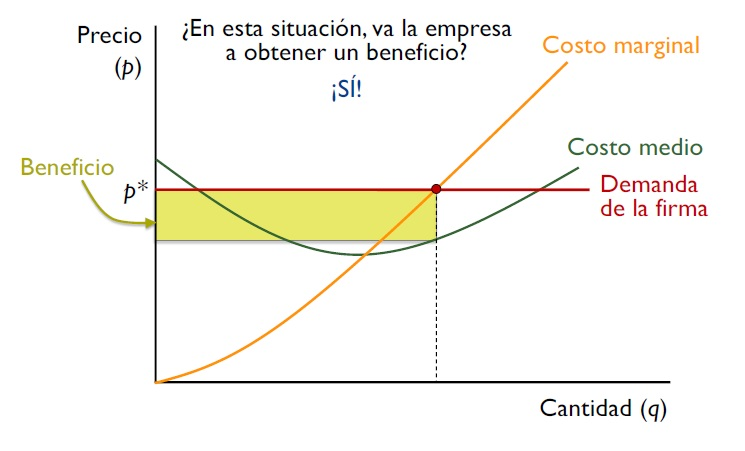
\includegraphics[scale=0.55]{Slides Principios de Economia/Figures/Tema_07.11_compperfecta5.jpg}
\end{frame}

\begin{frame}
\frametitle{¿Habrá beneficio en este punto? NO! ¿Hay perdida? SI!}
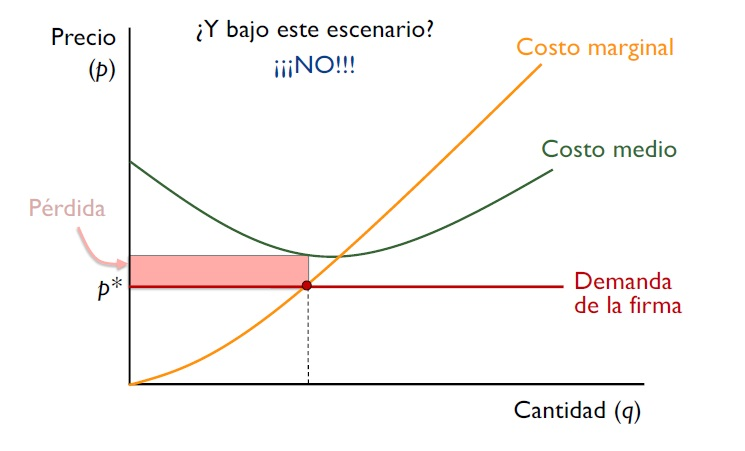
\includegraphics[scale=0.55]{Slides Principios de Economia/Figures/Tema_07.12_compperfecta6.jpg}
\end{frame}

\begin{frame}
\frametitle{¿Habrá beneficio extraordinario en este punto? NO! ¿Hay perdida? NO!}
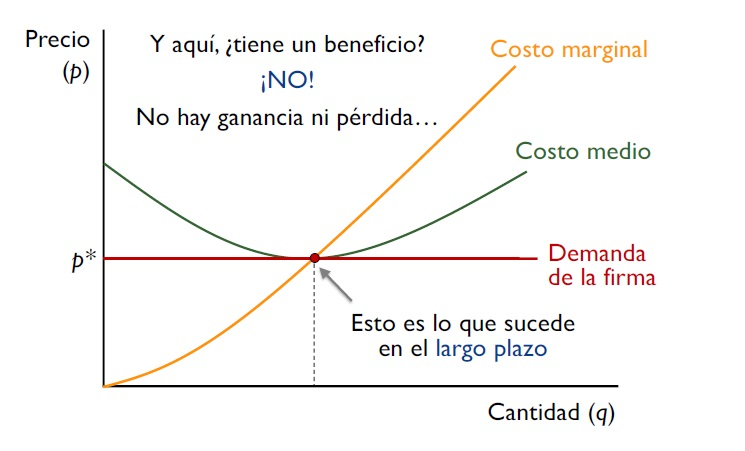
\includegraphics[scale=0.55]{Slides Principios de Economia/Figures/Tema_07.13_compperfecta7.jpg}
\end{frame}

\begin{frame}
\frametitle{Entonces en el CP....}
\centering
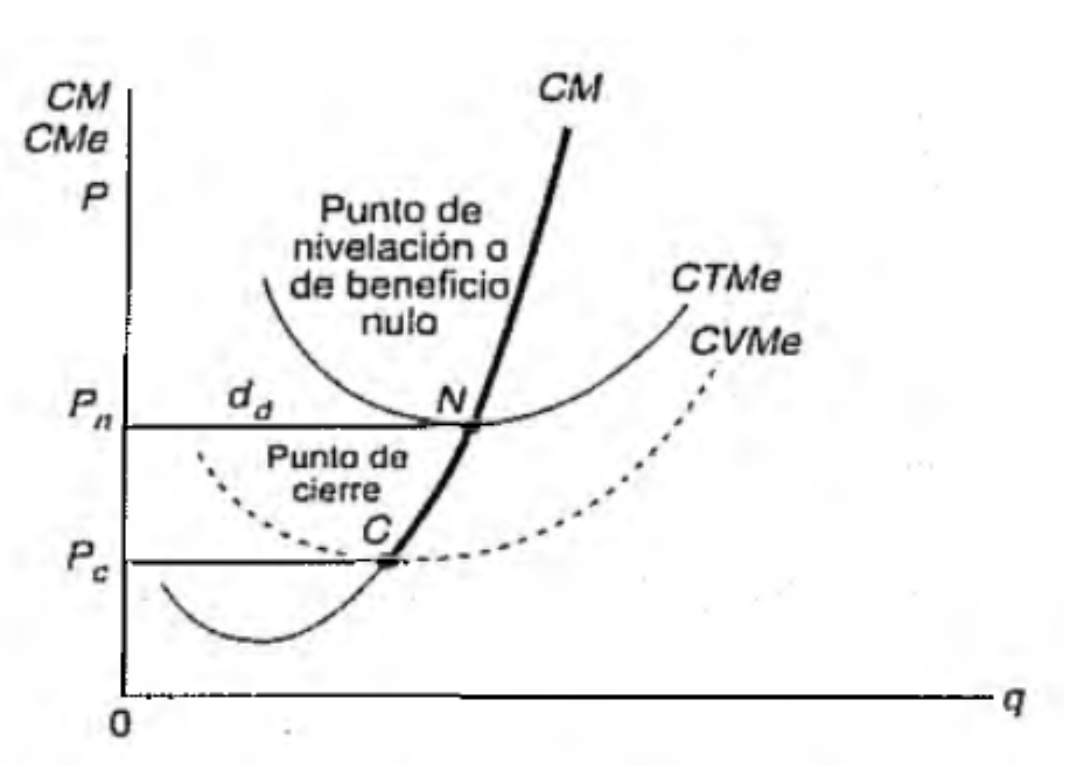
\includegraphics[scale=0.85]{Slides Principios de Economia/Figures/ZonasCP.png}
\end{frame}


\begin{frame}
\frametitle{¿Y en el largo plazo...}
\begin{itemize}
    \item Siempre que existan potenciales rentas (beneficios extraordinarios), va a haber firmas interesadas en entrar al mercado
    \item Si los costos de entrada no son demasiado altos, estas firmas potenciales van a entrar
    \item Al ingresar, las firmas van a presionar hacia abajo el precio de equilibrio, eliminando del mercado a las firmas menos eficientes
    \item Los beneficios que atraen a potenciales entrantes comienzan a disiparse
    \item En el largo plazo, estos beneficios van a desaparecer, serán iguales a 0
    \end{itemize}
\end{frame}

\begin{frame}
\frametitle{¿Y en el largo plazo...}
\begin{center}
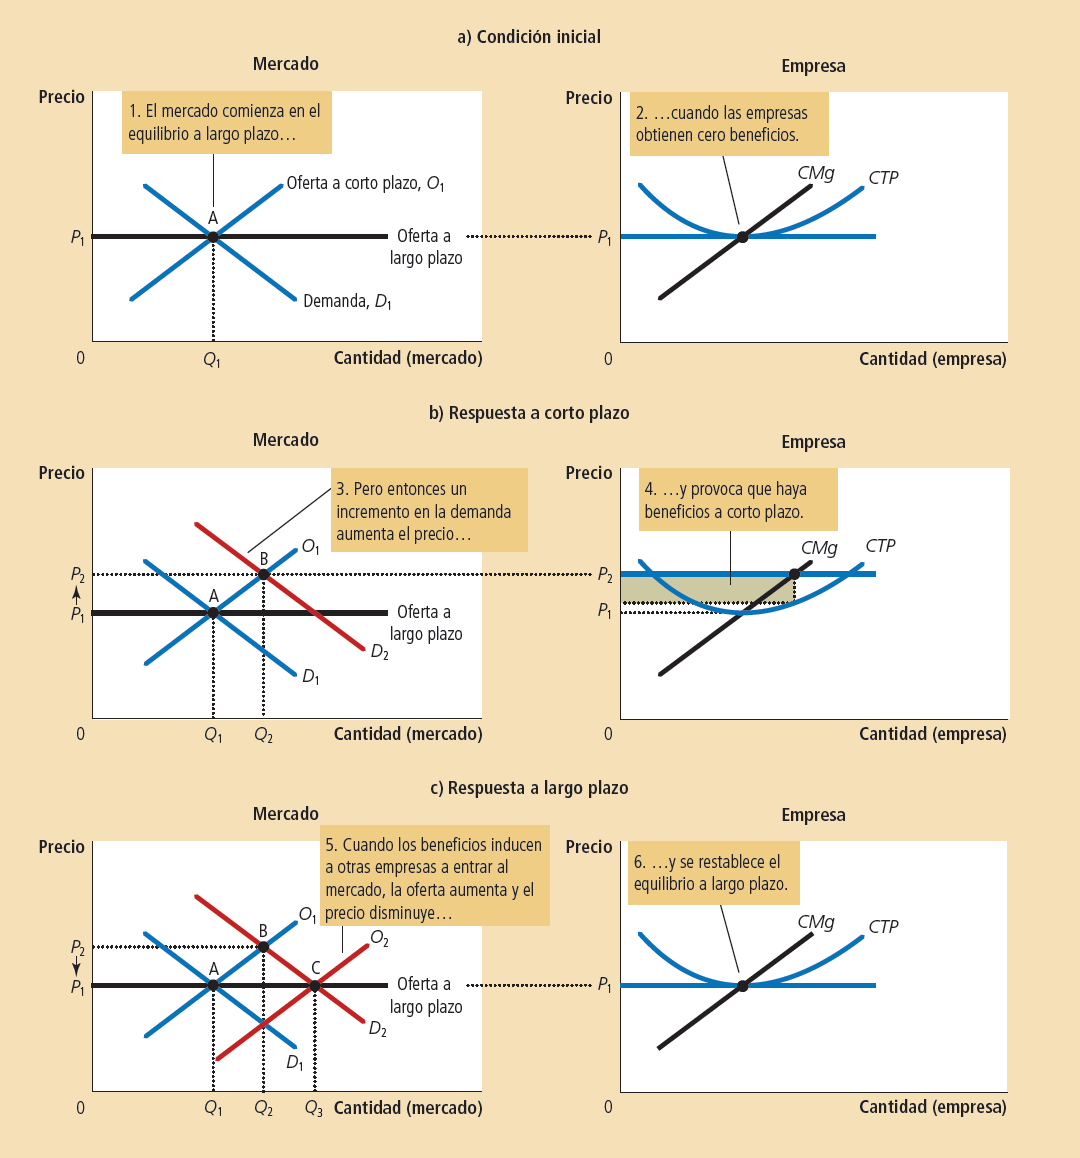
\includegraphics[scale=0.65]{Slides Principios de Economia/Figures/LargoplazoCP.png}
\end{center}
\end{frame}


\begin{frame}
\frametitle{Recordemos lo que sucede en equilibrio... beneficios para todos!}
\begin{center}
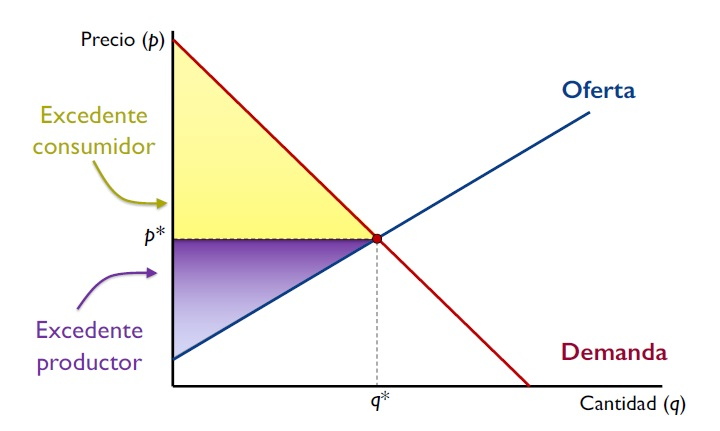
\includegraphics[scale=0.55]{Slides Principios de Economia/Figures/Tema_07.23_equilibrioyexcedente.jpg}
\end{center}
\end{frame}

\begin{frame}
\frametitle{¿Por qué es eficiente?}
\begin{itemize}
    \item Los participantes son tomadores de precios\vspace{2mm}
    \begin{itemize}
        \item No hay poder de mercado.\vspace{1mm}
        \item La competencia impide a los vendedores aumentar el precio, y a los compradores bajarlo.\vspace{2mm}
    \end{itemize}
    \item Los contratos son completos\vspace{2mm}
        \begin{itemize}
        \item Los detalles del intercambio pueden ser definidos en forma clara, y estos contratos se pueden hacer cumplir.\vspace{2mm}
        \end{itemize}
    \item No hay externalidades\vspace{2mm}
        \begin{itemize}
        \item La transacción sólo afecta a los compradores y vendedores
        \end{itemize}
\end{itemize}
\end{frame}

\begin{frame}
\frametitle{Resumen...}
\small
\begin{center}
    \begin{tabular}{c|c}
    \hline
    \hline
    Tomadores de precios & Fijadores de precio \\
    Competencia Perfecta & Monopolio
    \\
    \hline
    \hline
    Puede ser   &  \\ 
    Pareto eficiente & 
    \\
    \hline
    No hay rentas &  \\
    económicas en &  \\
    el largo plazo & 
    \\
    \hline
    Poca gasto en su &  \\ publicidad & 
    \\
    \hline
    Pocos incentivos para &   \\ 
    la innovación porque &  \\
    porque otras van a copiar & 
\end{tabular}
\end{center}
\end{frame}


\end{document}
